% Conference deck for "No Universal AI Dominance".
% Build:  tectonic -X compile slides.tex
% Figures are the same PDFs the article uses, from figs/.
\documentclass[aspectratio=169,11pt]{beamer}
\usepackage[utf8]{inputenc}
\usepackage[T1]{fontenc}
\usepackage{lmodern}
\usepackage{booktabs}
\usepackage{amsmath,amssymb}
\usepackage{xcolor}

\usetheme{default}
\usefonttheme{professionalfonts}
\setbeamertemplate{navigation symbols}{}
\setbeamertemplate{itemize items}[circle]

\definecolor{ink}{HTML}{14213D}
\definecolor{accent}{HTML}{BC4749}
\definecolor{mid}{HTML}{5A6B8C}
\definecolor{pale}{HTML}{EDF2F7}

\setbeamercolor{structure}{fg=ink}
\setbeamercolor{frametitle}{fg=ink,bg=white}
\setbeamercolor{normal text}{fg=ink}
\setbeamercolor{alerted text}{fg=accent}
\setbeamerfont{frametitle}{series=\bfseries,size=\large}
\setbeamertemplate{frametitle}{\vspace{0.6em}\insertframetitle\par\vspace{-0.4em}%
  {\color{ink!25}\rule{\textwidth}{0.6pt}}}
\setbeamertemplate{footline}{%
  \hfill{\tiny\color{mid}\insertframenumber}\hspace{1.2em}\vspace{0.6em}}

\newcommand{\lead}[1]{{\color{accent}\textbf{#1}}}
\newcommand{\punch}[1]{\vspace{0.6em}{\color{mid}\small #1}}

\title{\textbf{No Universal AI Dominance}}
\subtitle{A multi-dimensional falsification test of vendor, paradigm and origin dominance in global LLM adoption}
\author{Rodrigo F. A. P. Oliveira}
\institute{\small CESAR School, Recife, Brazil \\ \texttt{rfapo@cesar.school}}
\date{\small November 2026}

\begin{document}

\begin{frame}[plain]
  \titlepage
  \vfill
  {\footnotesize\color{mid} Data, code and the full test suite:
   \texttt{github.com/rfapo/no-universal-ai-dominance}}
\end{frame}

% ---------------------------------------------------------------- the puzzle
\begin{frame}{Three claims, three answers, same market}
  \vspace{0.4em}
  \begin{columns}[T]
    \column{0.48\textwidth}
      \textbf{Web traffic} \\
      \punch{ChatGPT took 77\% of visits to the top 60 generative AI tools (2025); US models about 93\% of global LLM site visits.}
      \vspace{1.1em}

      \textbf{Gateway telemetry} \\
      \punch{Open-weight models from Chinese labs process most tokens.}
      \vspace{1.1em}

      \textbf{Enterprise spend} \\
      \punch{A third ranking entirely, led by Anthropic.}
    \column{0.48\textwidth}
      \vspace{2em}
      \begin{beamercolorbox}[wd=\textwidth,sep=1em]{postit}
        \color{ink}
        These are compatible \emph{only} if ``dominance'' depends on what is counted.
        \vspace{0.8em}

        \lead{So: is there any definition-robust dominance in LLM adoption?}
      \end{beamercolorbox}
  \end{columns}
\end{frame}

% ---------------------------------------------------------------- design
\begin{frame}{Design: make dominance the \emph{null}}
  \vspace{0.3em}
  Usual practice makes ``no effect'' the null, so failing to detect dominance says nothing.
  We reverse the burden of proof, as in equivalence testing.
  \vspace{0.9em}

  \begin{center}
  \begin{minipage}{0.86\textwidth}
  \begin{align*}
    H_0(\tau):\quad & \exists\, v \;\; \forall\, d \in \{A,\dots,E\}: \; s_{v,d} \ge \tau
      && \text{\small universal dominance}\\[2pt]
    H_1(\tau):\quad & \forall\, v \;\; \exists\, d: \; s_{v,d} < \tau
      && \text{\small no universal dominance}
  \end{align*}
  \end{minipage}
  \end{center}
  \vspace{0.6em}

  \begin{itemize}\setlength\itemsep{0.35em}
    \item $\tau = 50\%$ primary (EU case law); 40\% and 30\% as sensitivity
    \item Union--intersection over dimensions, intersection--union over vendors
    \item \lead{The data must be shown incompatible with dominance}, not merely silent on it
  \end{itemize}
\end{frame}

\begin{frame}{Five dimensions, five different units}
  \vspace{0.6em}
  \begin{center}\small
  \begin{tabular}{@{}llll@{}}
    \toprule
    & Dimension & Unit & Who is being counted \\
    \midrule
    A & Consumer attention & web visits      & visitors \\
    B & User base          & monthly actives & accounts, devices \\
    C & Revenue            & US dollars      & payers \\
    D & Developer volume   & requests, tokens& applications \\
    E & Enterprise spend   & US dollars      & firms \\
    \bottomrule
  \end{tabular}
  \end{center}
  \vspace{0.9em}
  \punch{Plus independent second sources (D$'$, E$'$, F) and one regional metric (G).
  Nine share metrics over 61 data sources and 53 scholarly works, at three levels:
  vendor, paradigm (closed vs open weights) and origin (US vs China).}
\end{frame}

% ---------------------------------------------------------------- results
\begin{frame}{Result 1: the leader changes with the unit}
  \vspace{-0.6em}
  \begin{center}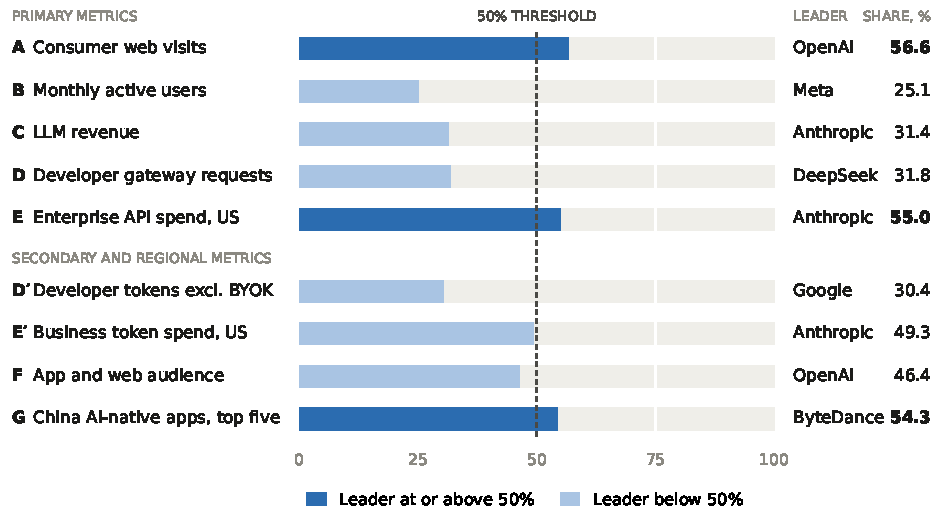
\includegraphics[width=0.80\textwidth]{figs/fig_leader.pdf}\end{center}
  \vspace{-0.6em}
  \punch{Nine metrics, \lead{six different leaders}.}
\end{frame}

\begin{frame}{Result 2: no uniformly dark row}
  \vspace{-0.2em}
  \begin{center}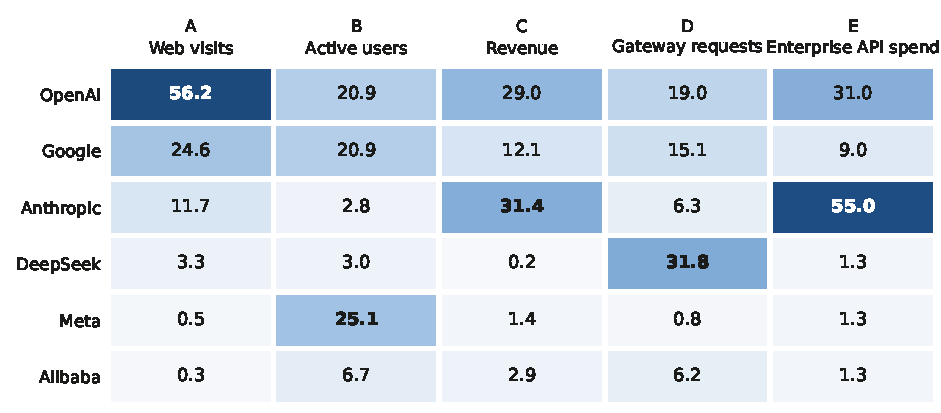
\includegraphics[width=0.90\textwidth]{figs/fig_heatmap.pdf}\end{center}
  \vspace{-0.4em}
  \punch{Universal dominance would be one row dark across every column.
  \lead{No vendor reaches 50\% in more than one of five dimensions.} Four vendors lead the five.}
\end{frame}

\begin{frame}{Result 3: the calibrated test}
  \vspace{0.3em}
  $T_v(\tau)=\sum_d \max\{0,\ln(\tau/s_{v,d})\}$, evaluated at the least favourable point of $H_0$.
  \vspace{0.8em}
  \begin{center}\small
  \begin{tabular}{@{}lrrr@{}}
    \toprule
    Specification & $\tau$ & $p$ (independent) & $p$ (correlated) \\
    \midrule
    Primary matrix            & 50 & \lead{0.0002} & \lead{0.018} \\
    Primary matrix            & 40 & 0.010 & 0.076 \\
    Primary matrix            & 30 & 0.33  & 0.32 \\
    \addlinespace
    Most favourable to $H_0$  & 50 & 0.074 & 0.161 \\
    \bottomrule
  \end{tabular}
  \end{center}
  \vspace{0.8em}
  \punch{On single-source data $H_0(50)$ is rejected, and survives error scales up to
  $\sigma=0.65$ (95\% of errors within a factor of 3.6). \lead{The error model is assumed,
  not estimated}, so the whole $\sigma$ curve is reported, not one number.}
\end{frame}

% ---------------------------------------------------------------- honesty
\begin{frame}{Where the null is \emph{not} rejected}
  \vspace{0.2em}
  A title like ours is easy to over-read. Reported with equal weight:
  \vspace{0.7em}
  \begin{itemize}\setlength\itemsep{0.45em}
    \item \textbf{Most favourable reading.} Take the largest share any source reports in every
      cell and $p$ rises to \lead{0.07--0.16}. The rejection fails.
    \item \textbf{Ownership blocs.} Count Google and Anthropic as one (13.7\% stake) and a
      \lead{30\% threshold is met in all five dimensions}.
    \item \textbf{Asymmetry.} Dominance by \emph{open weights} and by \emph{Chinese labs} is
      rejected; by \emph{closed weights} and \emph{US labs} it is \lead{not}.
    \item \textbf{Concentration is real.} HHI above 1{,}800 in six of nine metrics.
      This is not a finding that the market is competitive.
    \item \textbf{Upstream is another market.} One firm holds \lead{75--86\%} of AI accelerators.
  \end{itemize}
\end{frame}

% ---------------------------------------------------------------- open weights
\begin{frame}{The sharpest result: author $\neq$ seller}
  \vspace{0.6em}
  Anyone may serve released weights, so ``who made it'' and ``who sells it'' are different firms.
  \vspace{1.0em}
  \begin{center}
  \begin{tabular}{@{}lcc@{}}
    \toprule
    Same tokens, attributed to\dots & HHI & effective competitors \\
    \midrule
    the \textbf{model family} & 3{,}225 & 3.1 \\
    the \textbf{seller}       &   559  & 17.9 \\
    \bottomrule
  \end{tabular}
  \end{center}
  \vspace{1.0em}
  \punch{Highly concentrated, or unconcentrated, on \emph{identical data}.
  Chinese families supply \lead{89.6\%} of open-weight gateway tokens while
  \lead{57.6\%} of those tokens are sold by US-headquartered firms.}
\end{frame}

\begin{frame}{Durability points two ways}
  \vspace{-0.3em}
  \begin{center}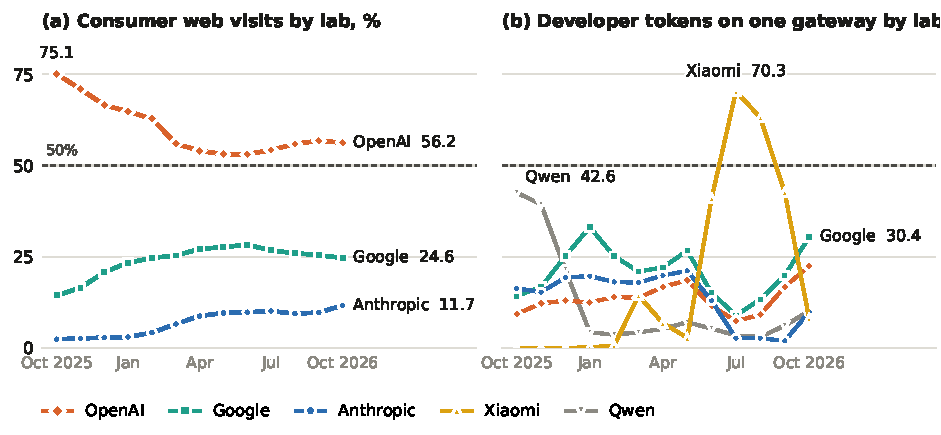
\includegraphics[width=0.66\textwidth]{figs/fig_panel.pdf}\end{center}
  \vspace{-0.5em}
  \begin{center}\small
  \begin{tabular}{@{}lcc@{}}
    \toprule
     & Consumer visits & Developer tokens \\
    \midrule
    Distinct leaders in 13 months & 1 & \lead{3} \\
    Months with leader $\ge 50\%$ & \lead{13} & 2 \\
    Market changing hands / month & 2.9\% & \lead{19.4\%} \\
    \bottomrule
  \end{tabular}
  \end{center}
  \vspace{-0.2em}
  \punch{Thirteen months cannot identify tipping dynamics, so this stays descriptive.}
\end{frame}

% ---------------------------------------------------------------- multi-homing
\begin{frame}{What a share cannot tell you}
  \vspace{0.5em}
  A share counts a multi-homing user once per brand. How much of the leader's base is
  \emph{exclusive}? The mean of 1.49 tools per user cannot say, but the marginals bound it.
  \vspace{0.7em}
  \begin{center}
  $e \ge A - \textstyle\sum_k r_k \qquad\text{and}\qquad e \le A - \max_k r_k$
  \end{center}
  \vspace{0.7em}
  \begin{center}\small
  \begin{tabular}{@{}lc@{}}
    \toprule
    Leader's raw share of users & 66.7\% \\
    Share genuinely exclusive & \lead{between 17.6\% and 52.9\%} \\
    \bottomrule
  \end{tabular}
  \end{center}
  \vspace{0.8em}
  \punch{Both bounds sharp, verified by linear programming over user types.
  The interval is wide and that \emph{is} the result: survey marginals cannot say whether a
  quarter or four fifths of the base is captive. Only that the share overstates dependence.}
\end{frame}

% ---------------------------------------------------------------- takeaway
\begin{frame}{What to take away}
  \vspace{0.8em}
  \begin{beamercolorbox}[wd=\textwidth,sep=1.1em]{box}
    \color{ink}\large
    A claim of dominance should name its \lead{unit}, its \lead{market} and its \lead{source}.
  \end{beamercolorbox}
  \vspace{1.0em}
  \begin{itemize}\setlength\itemsep{0.4em}
    \item \textbf{Measurement.} Token share is not market share. It moved tens of points in a
      quarter under price promotions, and differs from spend share by exactly the price gap ($\approx 7\times$).
    \item \textbf{Policy.} The antitrust question is segment-specific: strongest for consumer
      chat and enterprise APIs, weakest for developer inference.
    \item \textbf{Diffusion.} The sharper divide is between populations, not vendors: 12.6 points
      between Global North and South; 53 points between Brazil's top and bottom income classes.
  \end{itemize}
\end{frame}

\begin{frame}{Everything here is reproducible}
  \vspace{0.7em}
  \begin{itemize}\setlength\itemsep{0.45em}
    \item Every transcribed input lives inline in \texttt{code/analysis.py} beside its citation;
      there is no hidden dataset.
    \item \texttt{results.json} reproduces \lead{byte for byte} on Linux and macOS; CI re-runs the
      whole analysis on every push.
    \item \texttt{validate\_stats.py} re-derives each procedure by a different route:
      Kendall's $W$ via Friedman, the HHI bound against brute force, the exclusivity interval by linear programming.
    \item \lead{103 tests} hold every number in the paper against \texttt{results.json}.
    \item Data are secondary and several sources are live dashboards: 46 of 63 URLs carry a
      snapshot no older than the month they were read. We say which do not.
  \end{itemize}
  \vspace{0.9em}
  \begin{center}\small\texttt{github.com/rfapo/no-universal-ai-dominance}\end{center}
\end{frame}

\begin{frame}[plain]
  \vspace{2.2em}
  \begin{center}
    {\Large\textbf{No Universal AI Dominance}}\\[0.9em]
    {\color{mid} There is no single market here, and no single leader.}\\[0.4em]
    {\color{mid} There are segments, each concentrated, each led by someone else.}\\[2.0em]
    {\small Rodrigo F. A. P. Oliveira \quad\textbar\quad \texttt{rfapo@cesar.school}}\\[0.5em]
    {\footnotesize\color{mid}\texttt{github.com/rfapo/no-universal-ai-dominance}}
  \end{center}
\end{frame}

\end{document}
